\documentclass[]{standalone}
\usepackage{tikz}
\usetikzlibrary{shapes,arrows,calc,positioning}
\usepackage{amsmath} % for dfrac
\usepackage{comment}
\usepackage{calc}

% definition of basic block
\tikzset{
    block/.style = {draw, rectangle,
        minimum height=1.2cm,
        minimum width=2cm},
    input/.style = {coordinate,node distance=1cm},
    output/.style = {coordinate,node distance=1cm},
    sum/.style = {draw, circle, node distance=1cm},
}

% definition of saturation block
\tikzset{% from https://tex.stackexchange.com/questions/161075/saturation-block
  saturation block/.style={%
    draw, 
    path picture={
      % Get the width and height of the path picture node
      \pgfpointdiff{\pgfpointanchor{path picture bounding box}{north east}}%
        {\pgfpointanchor{path picture bounding box}{south west}}
      \pgfgetlastxy\x\y
      % Scale the x and y vectors so that the range
      % -1 to 1 is slightly shorter than the size of the node
      \tikzset{x=\x*.4, y=\y*.4}
      %
      % Draw annotation
      \draw (-1,0) -- (1,0) (0,-1) -- (0,1); 
      \draw (-1,-.7) -- (-.6,-.7) -- (.6,.7) -- (1,.7);
    }
  }
}
\tikzset{% from https://tex.stackexchange.com/questions/161075/saturation-block
  deadband block/.style={%
    draw, 
    path picture={
      % Get the width and height of the path picture node
      \pgfpointdiff{\pgfpointanchor{path picture bounding box}{north east}}%
        {\pgfpointanchor{path picture bounding box}{south west}}
      \pgfgetlastxy\x\y
      % Scale the x and y vectors so that the range
      % -1 to 1 is slightly shorter than the size of the node
      \tikzset{x=\x*.4, y=\y*.4}
      %
      % Draw annotation
      \draw (-1,0) -- (1,0) (0,-1) -- (0,1);  % axis
      \draw (-1,1) -- (-.3,.3) -- (-.3,0) -- (.3,0) -- (.3,-.3) -- (1,-1);
	  %\draw (-.3,.3) -- (.3,-.3) ;
    }
  }
}

\begin{document}
	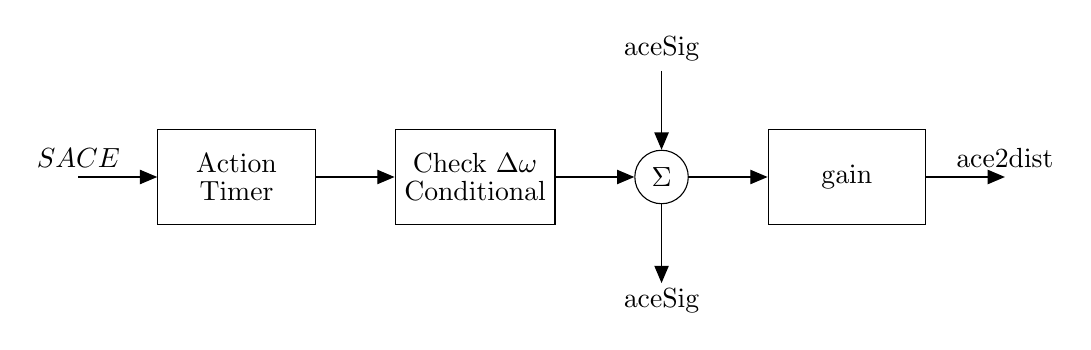
\begin{tikzpicture}[auto, node distance=1cm,>=triangle 45]
		% Starting inputwref
		\node [input, name=inputSACE, label=$SACE$]  {};
		
		\node [block, right=of inputSACE,] (timer) {\shortstack{Action\\Timer}};
		
		\node [block, right=of timer,] (conditional) {\shortstack{Check $\Delta\omega$\\Conditional}};
		
				
		\node [sum, right =of conditional] (ace2distSum) {$\Sigma$};
		\node [input, above = of ace2distSum, name=aceSigInput, label=aceSig]  {};
		\node [output, below = of ace2distSum, name=aceSigOutput]  {};
		\coordinate [below=0.5cm of aceSigOutput,label=aceSig]  (outputlabel){};
		
		\node [block, right=of ace2distSum] (gain) {gain};
		
		\node [output, right=of gain, label=ace2dist] (output) {};
		
		%% connecting lines
		\draw [->] (inputSACE) -- (timer);
		\draw [->] (timer) -- (conditional);
		\draw [->] (conditional) -- (ace2distSum);
		\draw [->] (ace2distSum) -- (gain);
		\draw [->] (gain) -- (output);
		
		\draw [->] (aceSigInput) -- (ace2distSum);
		\draw [->] (ace2distSum) -- (aceSigOutput) [coordinate, label=aceSig, anchor=south] ;

	\end{tikzpicture} 
\end{document}